\chapter{Translational Kinematics}
\label{ch:kine}


\textit{I can calculate the movement of the stars, but not the madness of men.}  \\
\noindent\textbf{-Isaac Newton}

\begin{marginfigure}[0pt]%
  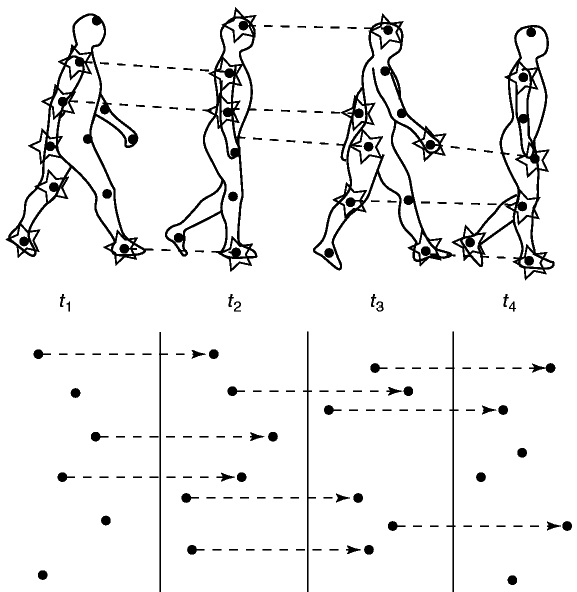
\includegraphics[width=\linewidth]{tseries.jpg}
  \caption{Time series of human motion}
  \label{fig:marginfig}
\end{marginfigure}

\marginnote[300pt]{
In Euclidean geometry, a translation is a function that moves every point a constant distance in a specified direction.  A translation can be described as a rigid motion: other rigid motions include rotations and reflections. A translation can also be interpreted as the addition of a constant vector to every point, or as shifting the origin of the coordinate system.}




\vspace{1cm}


\section{Translational Motion in Space and Time}
Translation is the movement associated with a point particle.  An extended body can have rotational motion and deformations.  When a particle moves through space we describe its motion by collecting ordered pairs of position vectors and times.  This is known as a time series.  Algebraically this corresponds to and x,y,z and t value.  Geometrically this is equivalent to a point in space and a point in time.  These pairs can be considered part of a continuos function.



$$\{\overrightarrow{\scriptr},t\}\ni\overrightarrow{\scriptr}(t)$$

\begin{figure}%

\tdplotsetmaincoords{60}{110}
$$\begin{tikzpicture}[scale=1,tdplot_main_coords]
\coordinate (O) at (0,0,0);
\coordinate (P) at (1,2,3);

\draw[thick,->] (0,0,0) -- (4,0,0) node[anchor=north east]{$x$};
\draw[thick,->] (0,0,0) -- (0,4,0) node[anchor=north west]{$y$};
\draw[thick,->] (0,0,0) -- (0,0,4) node[anchor=south]{$z$};

%draw a vector from origin to point (P) 
\draw[-stealth,very thick,color=red] (O) -- (P) node[anchor=south,color=black]{$\overrightarrow{\scriptr}(t)$};


%draw projection on xy plane, and a connecting line
%syntax: \tdplotdrawarc[coordinate frame, draw options]{center point}{r}{angle}{label options}{label}
%\tdplotdrawarc{(O)}{0.2}{0}{\phivec}{anchor=north}{$\phi$}


%set the rotated coordinate system so the x'-y' plane lies within the
%"theta plane" of the main coordinate system
%syntax: \tdplotsetthetaplanecoords{\phi}
%\tdplotsetthetaplanecoords{\phivec}

%draw theta arc and label, using rotated coordinate system
%\tdplotdrawarc[tdplot_rotated_coords]{(0,0,0)}{0.5}{0}{\thetavec}{anchor=south west}{$\theta$}

\end{tikzpicture}
\hspace{1cm}
\begin{tikzpicture}[scale=1.2]
\draw[thick,->,white] (0,0) -- (4,0) node[anchor=north]{$t$};
\draw[thick,-latex] (0,2) -- (4,2) node[anchor=north]{$t$};
\fill[black] (0.25,2) circle (0.5mm) node [anchor=south ,scale=1] {$0$};
    \fill[black] (2.25,2) circle (0.5mm) node [anchor=south ,scale=1] {$t$};
\end{tikzpicture}$$


  \caption{Geometric position and time}
  \label{fig:marginfig}
\end{figure}


\subsection{Displacement and Time Lapse}
Applying the delta operator $\Delta$ to spatial vector and time series yields the displacement vector and elapsed time.  The vector difference between points in space is known as displacement.  In the temporal dimension the difference between points represents time elapsed.
\begin{marginfigure}[0pt]%
  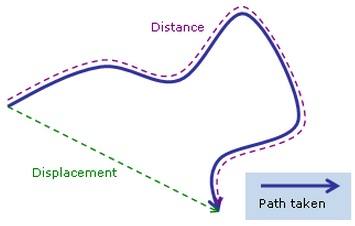
\includegraphics[width=\linewidth]{disp.jpg}
  \caption{Displacement, path and distance traveled}
  \label{fig:marginfig}
\end{marginfigure}
$$\Delta \overrightarrow{\scriptr}=\overrightarrow{\scriptr}_b-\overrightarrow{\scriptr}_a$$
$$\Delta t = t_b-t_a$$
A displacement is the shortest distance from the initial to the final position of a point.  Thus, it is the length of an imaginary straight path, typically distinct from the path actually travelled. A displacement vector represents the length and direction of this imaginary straight path.  A displacement may be also described as a 'relative position': the final position of a point relative to its initial position, and a displacement vector can be mathematically defined as the difference between the final and initial position vectors.




\begin{figure}
\tdplotsetmaincoords{60}{110}
$$\begin{tikzpicture}[scale=1,tdplot_main_coords]
\coordinate (O) at (0,0,0);
\coordinate (P) at (1,2,3);
\coordinate (T) at (1,3,2);

\draw[thick,->] (0,0,0) -- (4,0,0) node[anchor=north east]{$x$};
\draw[thick,->] (0,0,0) -- (0,4,0) node[anchor=north west]{$y$};
\draw[thick,->] (0,0,0) -- (0,0,4) node[anchor=south]{$z$};

%draw a vector from origin to point (P) 
\draw[-stealth,very thick,color=red] (P) -- (T) node[midway,anchor=south west,color=black]{\footnotesize$\Delta\overrightarrow{\scriptr}$};
\draw[-stealth,thick,color=red] (O) -- (T) node[anchor=north,color=black]{\footnotesize$\overrightarrow{\scriptr}_b$};
\draw[-stealth,thick,color=red] (O) -- (P) node[anchor=south east,color=black]{\footnotesize$\overrightarrow{\scriptr}_a$};


%draw projection on xy plane, and a connecting line
%syntax: \tdplotdrawarc[coordinate frame, draw options]{center point}{r}{angle}{label options}{label}
%\tdplotdrawarc{(O)}{0.2}{0}{\phivec}{anchor=north}{$\phi$}


%set the rotated coordinate system so the x'-y' plane lies within the
%"theta plane" of the main coordinate system
%syntax: \tdplotsetthetaplanecoords{\phi}
%\tdplotsetthetaplanecoords{\phivec}

%draw theta arc and label, using rotated coordinate system
%\tdplotdrawarc[tdplot_rotated_coords]{(0,0,0)}{0.5}{0}{\thetavec}{anchor=south west}{$\theta$}

\end{tikzpicture}
\hspace{1cm}
\begin{tikzpicture}[scale=1.2]
\draw[thick,->,white] (0,0) -- (4,0) node[anchor=north]{$t$};
\draw[thick,-latex] (0,2) -- (4,2) node[anchor=north]{$t$};
%\fill[black] (0.25,2) circle (0.5mm) node [anchor=north ,scale=1] {$0$};
    \fill[black] (2,2) circle (0.5mm) node [anchor=north ,scale=1] {$t_a$};
      \fill[black] (3,2) circle (0.5mm) node [anchor=north ,scale=1] {$t_b$};
      \draw[thick,->] (2,2.25) -- (3,2.25) node[midway,anchor=south]{\footnotesize$\Delta t$};
\end{tikzpicture}$$
 \caption{Geometric displacement and elapsed time}
  \label{fig:marginfig}
\end{figure}

Algebraically this corresponds to and $(\Delta x,\Delta y,\Delta z)$ and t value.  Geometrically this is equivalent to a vector in space and a elapse of time.
$$\Delta \overrightarrow{\scriptr}=\Delta x \hat{x}+\Delta y\hat{y}+\Delta z\hat{z}=\left(\begin{array}{c} \Delta x \\ \Delta y \\ \Delta z\end{array}\right)$$

\subsection{Average Velocity}
Average velocity is defined as the displacement vector divided by the elapsed time.  It is a time rate vector pointing in the direction of the displacement.
$$\bar{\overrightarrow{v}}=<\overrightarrow{v}>=\frac{\Delta \overrightarrow{\scriptr}}{\Delta t}$$


\begin{figure}
\tdplotsetmaincoords{60}{110}
$$\begin{tikzpicture}[scale=1,tdplot_main_coords]
\coordinate (O) at (0,0,0);
\coordinate (P) at (1,2,3);
\coordinate (T) at (1,2.4,2.6);

\draw[thick,->] (0,0,0) -- (4,0,0) node[anchor=north east]{$x$};
\draw[thick,->] (0,0,0) -- (0,4,0) node[anchor=north west]{$y$};
\draw[thick,->] (0,0,0) -- (0,0,4) node[anchor=south]{$z$};

%draw a vector from origin to point (P) 
\draw[-stealth,very thick,color=blue] (P) -- (T) node[midway,anchor=south west,color=black]{\footnotesize$\Delta\overrightarrow{\scriptr}=\braket{\overrightarrow{v}}(t) \Delta t$};
\draw[-stealth, thick,color=red] (O) -- (T) node[anchor=north west,color=black]{\footnotesize$\overrightarrow{\scriptr}(t+\Delta t)$};
\draw[-stealth, thick,color=red] (O) -- (P) node[anchor=east,color=black]{\footnotesize$\overrightarrow{\scriptr}(t)$};


%draw projection on xy plane, and a connecting line
%syntax: \tdplotdrawarc[coordinate frame, draw options]{center point}{r}{angle}{label options}{label}
%\tdplotdrawarc{(O)}{0.2}{0}{\phivec}{anchor=north}{$\phi$}


%set the rotated coordinate system so the x'-y' plane lies within the
%"theta plane" of the main coordinate system
%syntax: \tdplotsetthetaplanecoords{\phi}
%\tdplotsetthetaplanecoords{\phivec}

%draw theta arc and label, using rotated coordinate system
%\tdplotdrawarc[tdplot_rotated_coords]{(0,0,0)}{0.5}{0}{\thetavec}{anchor=south west}{$\theta$}

\end{tikzpicture}
\hspace{1cm}
\begin{tikzpicture}[scale=1.2]
\draw[thick,->,white] (0,0) -- (4,0) node[anchor=north]{$t$};
\draw[thick,-latex] (0,2) -- (4,2) node[anchor=north]{$t$};
%\fill[black] (0.25,2) circle (0.5mm) node [anchor=north ,scale=1] {\footnotesize$0$};
    \fill[black] (2,2) circle (0.5mm) node [anchor=north ,scale=1] {\footnotesize$t$};
      \fill[black] (2.4,2) circle (0.5mm) node [anchor=north west ,scale=1] {\footnotesize$t+\Delta t$};
      \draw[thick,->] (2,2.25) -- (2.4,2.25) node[midway,anchor=south]{\footnotesize$\Delta t$};
\end{tikzpicture}$$
 \caption{Geometric displacement as average velocity times elapsed time}
  \label{fig:marginfig}
\end{figure}

Position is described by a three dimensional vector space.  Velocity too can be described by a three dimensional vector space.  The dimensions of velocity space are distance over time.  Since they are distant we should not technically draw a velocity vector on a position graph.  

\marginnote[-140pt]{An instant, $\lim \Delta t \rightarrow 0$, is an infinitesimal moment in time, a moment whose passage is instantaneous.  The continuous nature of time and its infinite divisibility was addressed by Aristotle in his Physics, where he wrote on Zeno's paradoxes. Scientists, philosophers and artists still seek to define the exact nature of an instant thousands of years later.\\

In physics, a theoretical lower-bound unit of time called the Planck time has been proposed, that being the time required for light to travel a distance of 1 Planck length. The Planck time is theorized to be the smallest time measurement that will ever be possible, roughly $10^{-43}$ seconds. Within the framework of the laws of physics as they are understood today, for times less than one Planck time apart, we can neither measure nor detect any change. As of May 2010, the smallest time interval that was directly measured was on the order of 12 attoseconds ($12 \times 10^{-18}$ seconds), about 1024 times larger than the Planck time. It is therefore physically impossible, with current technology, to determine if any action exists that causes a reaction in "an instant", rather than a reaction occurring after an interval of time too short to observe or measure.}

\subsection{Instantaneous Velocity}
Instantaneous velocity is defined as the average velocity in the limit as ${\Delta t}$ and $\Delta \overrightarrow{\scriptr}$ go to zero.  This is informally notated as $\Delta \rightarrow 0$.
$$\overrightarrow{v}=\lim_{\Delta \rightarrow 0}\frac{\Delta \overrightarrow{\scriptr}}{\Delta t}$$
The instantaneous velocity vector $\overrightarrow{v}$ has a component in the x, y and z directions.
$$\overrightarrow{v}=v_x\hat{x}+v_y\hat{y}+v_z\hat{z}=\left(\begin{array}{c} v_x \\ v_y \\ v_z\end{array}\right)$$

\newpage


\subsection{Change in Velocity}

Applying the delta operator $\Delta$ to the velocity vector yields a change in velocity vector $\Delta \overrightarrow{v}$.  The vector $\Delta \overrightarrow{v}$ is the difference between final velocity state and initial velocity state.  Algebraically this is the final velocity vector $\overrightarrow{v}_b$ minus the initial velocity vector $\overrightarrow{v}_a$.   
$$\Delta \overrightarrow{v}=\overrightarrow{v}_b-\overrightarrow{v}_a$$
Geometrically the change in velocity vector $\Delta \overrightarrow{v}$ represents the vector beginning at the point represented by $\overrightarrow{v}_a$ and ending at $\overrightarrow{v}_b$.  
\begin{figure}
$$\begin{tikzpicture}[scale=1,tdplot_main_coords]


\coordinate (O) at (0,0,0);
\coordinate (P) at (1,2,-3);
\coordinate (T) at (1,3,-2);

\draw[thick,->] (0,0,0) -- (4,0,0) node[anchor=north east]{$v_x$};
\draw[thick,->] (0,0,0) -- (0,4,0) node[anchor=north west]{$v_y$};
\draw[thick,->] (0,0,0) -- (0,0,4) node[anchor=south]{$v_z$};

%draw a vector from origin to point (P) 
\draw[-stealth,very thick,color=blue] (P) -- (T) node[midway,anchor=north west,color=black]{\footnotesize$\Delta\overrightarrow{v}$};
\draw[-stealth,thick,color=blue] (O) -- (T) node[anchor=west,color=black]{\footnotesize$\overrightarrow{v}_b$};
\draw[-stealth,thick,color=blue] (O) -- (P) node[anchor=east,color=black]{\footnotesize$\overrightarrow{v}_a$};


%draw projection on xy plane, and a connecting line
%syntax: \tdplotdrawarc[coordinate frame, draw options]{center point}{r}{angle}{label options}{label}
%\tdplotdrawarc{(O)}{0.2}{0}{\phivec}{anchor=north}{$\phi$}


%set the rotated coordinate system so the x'-y' plane lies within the
%"theta plane" of the main coordinate system
%syntax: \tdplotsetthetaplanecoords{\phi}
%\tdplotsetthetaplanecoords{\phivec}

%draw theta arc and label, using rotated coordinate system
%\tdplotdrawarc[tdplot_rotated_coords]{(0,0,0)}{0.5}{0}{\thetavec}{anchor=south west}{$\theta$}

\end{tikzpicture}
\hspace{1cm}
\begin{tikzpicture}[scale=1.2]
\draw[thick,->,white] (0,0) -- (4,0) node[anchor=north]{$t$};
\draw[thick,-latex] (0,2) -- (4,2) node[anchor=north]{$t$};
%\fill[black] (0.25,2) circle (0.5mm) node [anchor=north ,scale=1] {$0$};
    \fill[black] (2,2) circle (0.5mm) node [anchor=north ,scale=1] {$t_a$};
      \fill[black] (3,2) circle (0.5mm) node [anchor=north ,scale=1] {$t_b$};
      \draw[thick,->] (2,2.25) -- (3,2.25) node[midway,anchor=south]{\footnotesize$\Delta t$};
\end{tikzpicture}$$
 \caption{Geometric velocity and elapsed time}
  \label{fig:marginfig}
\end{figure}



\subsection{Average Acceleration}
Average acceleration is defined as the change in velocity vector divided by the elapsed time.  It is a time rate vector pointing in the direction of changing velocity.
$$\bar{\overrightarrow{a}}=<\overrightarrow{a}>=\frac{\Delta \overrightarrow{v}}{\Delta t}$$

\subsection{Instantaneous Acceleration}
Instantaneous acceleration is defined as the average acceleration in the limit as ${\Delta t}$ and $\Delta \overrightarrow{v}$ go to zero. 
$$\overrightarrow{a}=\lim_{\Delta \rightarrow 0}\frac{\Delta \overrightarrow{v}}{\Delta t}$$
The instantaneous acceleration is a vector with an x, y, and z component.
$$\overrightarrow{a}=a_x\hat{x}+a_y\hat{y}+a_z\hat{z}=\left(\begin{array}{c} a_x \\ a_y \\ a_z\end{array}\right)$$

\begin{figure}
\tdplotsetmaincoords{60}{110}
$$\begin{tikzpicture}[scale=1,tdplot_main_coords]
\coordinate (O) at (0,0,0);
\coordinate (P) at (1,2,-2);
\coordinate (T) at (1,2.4,-1.6);

\draw[thick,->] (0,0,0) -- (4,0,0) node[anchor=north east]{$v_x$};
\draw[thick,->] (0,0,0) -- (0,4,0) node[anchor=north west]{$v_y$};
\draw[thick,->] (0,0,0) -- (0,0,4) node[anchor=south]{$v_z$};

%draw a vector from origin to point (P) 
\draw[-stealth,very thick,color=green] (P) -- (T) node[midway,anchor=north west,color=black]{\footnotesize$\Delta \overrightarrow{v}=\braket{\overrightarrow{a}(t)} \Delta t$};
\draw[-stealth, thick,color=blue] (O) -- (T) node[anchor=south west,color=black]{\footnotesize$\overrightarrow{v}(t+\Delta t)$};
\draw[-stealth, thick,color=blue] (O) -- (P) node[anchor=east,color=black]{\footnotesize$\overrightarrow{v}(t)$};


%draw projection on xy plane, and a connecting line
%syntax: \tdplotdrawarc[coordinate frame, draw options]{center point}{r}{angle}{label options}{label}
%\tdplotdrawarc{(O)}{0.2}{0}{\phivec}{anchor=north}{$\phi$}


%set the rotated coordinate system so the x'-y' plane lies within the
%"theta plane" of the main coordinate system
%syntax: \tdplotsetthetaplanecoords{\phi}
%\tdplotsetthetaplanecoords{\phivec}

%draw theta arc and label, using rotated coordinate system
%\tdplotdrawarc[tdplot_rotated_coords]{(0,0,0)}{0.5}{0}{\thetavec}{anchor=south west}{$\theta$}

\end{tikzpicture}
\hspace{1cm}
\begin{tikzpicture}[scale=1.2]
\draw[thick,->,white] (0,0) -- (4,0) node[anchor=north]{$t$};
\draw[thick,-latex] (0,2) -- (4,2) node[anchor=north]{$t$};
\fill[black] (0.25,2) circle (0.5mm) node [anchor=north ,scale=1] {\footnotesize$0$};
    \fill[black] (2,2) circle (0.5mm) node [anchor=north ,scale=1] {\footnotesize$t$};
      \fill[black] (2.4,2) circle (0.5mm) node [anchor=north west ,scale=1] {\footnotesize$t+\Delta t$};
      \draw[thick,->] (2,2.25) -- (2.4,2.25) node[midway,anchor=south]{\footnotesize$\Delta t$};
\end{tikzpicture}$$
 \caption{Geometric position and time}
  \label{fig:marginfig}
\end{figure}

\begin{fullwidth}
In mathematics, infinitesimals are things so small that there is no way to measure them. The insight with exploiting infinitesimals was that entities could still retain certain specific properties, such as angle or slope, even though these entities were quantitatively small.  The word infinitesimal comes from a 17th-century Modern Latin coinage infinitesimus, which originally referred to the "infinite-th" item in a sequence. It was originally introduced around 1670 by either Nicolaus Mercator or Gottfried Wilhelm Leibniz.  Infinitesimals are a basic ingredient in the procedures of infinitesimal calculus as developed by Leibniz, including the law of continuity and the transcendental law of homogeneity. In common speech, an infinitesimal object is an object which is smaller than any feasible measurement, but not zero in size; or, so small that it cannot be distinguished from zero by any available means. Hence, when used as an adjective, "infinitesimal" means "extremely small". In order to give it a meaning it usually has to be compared to another infinitesimal object in the same context (as in a derivative). Infinitely many infinitesimals are summed to produce an integral.
\end{fullwidth}

\newpage
\section{Kinematic Difference: Slope and Curvature}
\begin{marginfigure}[20pt]%
  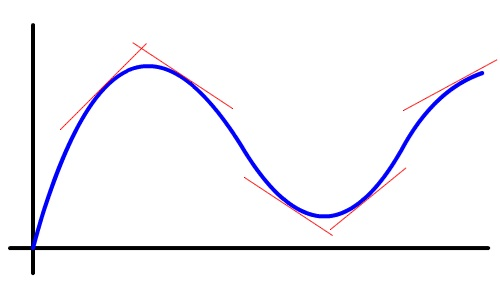
\includegraphics[width=\linewidth]{tangent.jpg}
  \caption{Tangent lines of a function}
  \label{fig:marginfig}
\end{marginfigure}
\subsubsection{Velocity}
In one dimensional motion there is only one degree of freedom, represented by the variable $x$.  When $x$ is graphed against $t$ in a position vs time graph the velocity is represented by the slope of the tangent line of $x(t)$.
$$v=\text{Slope of tangent line on position vs time graph}$$
$$v=\lim_{\Delta \rightarrow 0}\frac{\Delta x}{ \Delta t}$$
\begin{marginfigure}[40pt]%
  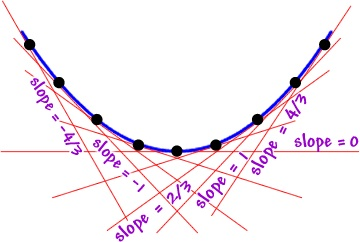
\includegraphics[width=\linewidth]{curve.jpg}
  \caption{Curvature of a function}
  \label{fig:marginfig}
\end{marginfigure}
\subsubsection{Acceleration}

When $v$ is graphed against $t$ in a velocity vs time graph the acceleration is represented by the slope of the tangent line of $v(t)$.  Acceleration is the time rate of change of the velocity.
$$a=\text{Slope of the tangent line on the velocity vs time graph}$$
$$a=\lim_{\Delta \rightarrow 0}\frac{\Delta v}{ \Delta t}$$
\begin{marginfigure}[60pt]%
  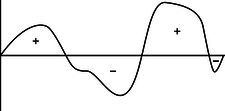
\includegraphics[width=\linewidth]{area.jpg}
  \caption{Area under a function}
  \label{fig:marginfig}
\end{marginfigure}
The acceleration is the rate of change of the velocity and the velocity is the slope of $x(t)$.  Therefore the acceleration is the rate of change of the slope, namely it is the curvature.
$$a=\text{Curvature on the position vs time graph}$$
$$a=\lim_{\Delta \rightarrow 0}\frac{\Delta \left( \nicefrac{\Delta x}{\Delta t}\right)}{ \Delta t}$$

\section{Kinematic Accumulation: Area Under Curve}
\subsubsection{Position}
\marginnote[30pt]{When $v$ is graphed against $t$ in a velocity vs time graph the displacement $\Delta x$ is the area under the graph of $v(t)$.  The displacement from the initial position $x(0)$ gives position as a function of time $x(t)$.}
$$\Delta x=\text{Area under velocity vs time graph}$$
$$\Delta x=\braket{v} \Delta t$$
$$x(t)=x(0)+\Delta x$$

\subsubsection{Velocity}
\marginnote[20pt]{When $a$ is graphed against $t$ in an acceleration vs time graph the change in velocity $\Delta v$ is the area under the graph of $a(t)$.  The change from the initial velocity $v(0)$ gives velocity as a function of time $v(t)$.}
$$\Delta v=\text{Area under acceleration vs time graph}$$
$$\Delta v=\braket{a} \Delta t$$
$$v(t)=v(0)+\Delta v$$



\newpage
\subsubsection{Graphical Representation}

\vspace{1cm}
\marginnote[50pt]{The slope of the tangent lines of the acceleration function is known as the jerk.  The area under the acceleration function is the change in velocity.  The change may be computed from the t=0 or an arbitrary time. }
\marginnote[125pt]{The slope of the tangent lines of the velocity function is the acceleration.  The area under the velocity function is the change in position, or displacement.  The change may be computed from the t=0 or an arbitrary time. }
\marginnote[125pt]{The slope of the tangent lines of the position function is the velocity.  The area under the position function is not physically meaningful. }
$$
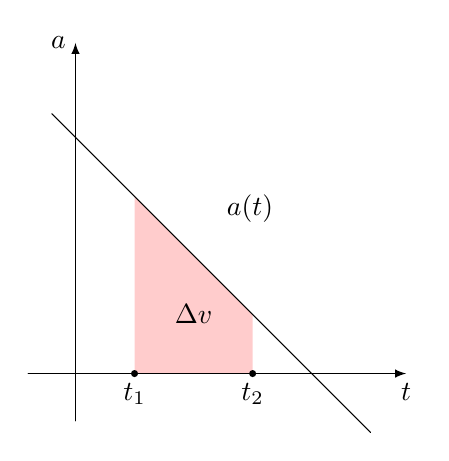
\begin{tikzpicture}
    [line cap=round,line join=round,x=2cm,y=2cm, scale=1.5, decoration={brace,amplitude=2pt}]
%main layer
%creating the ticks and xy-axis nodes
%some function
\fill[fill=red!20] (0.25,0) -- plot [domain=0.25:.75] (\x,{1-\x}) -- plot [domain=0.75: 0.25] (\x,0) -- cycle;

 \draw[smooth,samples=100,domain=-0.1:1.25]
                                 plot(\x,{1-\x});
 
  %\draw [darkgray,ultra thin] (0,0.479)-- (0.25,0.479);
  %\draw [darkgray,ultra thin] (0,0.938)-- (0.75,0.938);
 % \draw [darkgray,ultra thin] (0.25,0.479)-- (0.25,0.0);
  %\draw [darkgray,ultra thin] (0.75,0.938)-- (0.75,0);
%creating the curly braces with decorate
 
%  \draw [decorate,color=black!80!black] (0.25,0.0)--(0.75,0.0)
   %node [midway,anchor=north,inner sep=1pt, outer sep=1pt]{\small$\Delta x$};
    \fill[black] (0.25,0) circle (0.3mm) node [anchor=north ,scale=1] {$ t_1$};
     \fill[black] (0.75,0) circle (0.3mm) node [anchor=north ,scale=1] {$t_2$};

  \draw[-latex,color=black,thin] (-0.2,0) -- (1.4,0) node [anchor=north ,scale=1] {$t$};
   \draw[-latex,color=black,thin] (0,-0.2) -- (0,1.4)node [anchor=east ,scale=1] {$a$};
    \draw (0.6,0.6) node [anchor=south west ,scale=1] {$a(t)$};
        \draw (0.5,0.25) node [anchor=center ,scale=1] {$\Delta v$};
        
 \end{tikzpicture}
 \hspace{1cm}
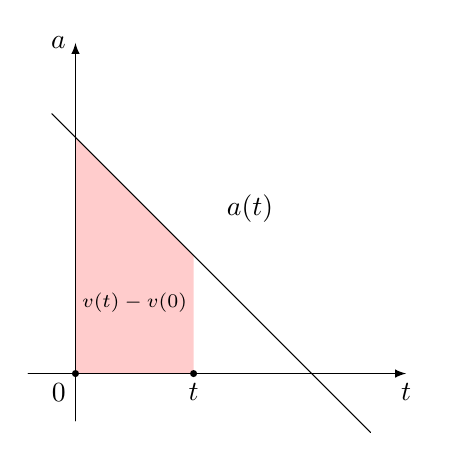
\begin{tikzpicture}
    [line cap=round,line join=round,x=2cm,y=2cm, scale=1.5, decoration={brace,amplitude=2pt}]
%main layer
%creating the ticks and xy-axis nodes
%some function
\fill[fill=red!20] (0,0) -- plot [domain=0:.5] (\x,{1-\x}) -- plot [domain=0.5: 0.0] (\x,0) -- cycle;

 \draw[smooth,samples=100,domain=-0.1:1.25]
                                 plot(\x,{1-\x});
 
  %\draw [darkgray,ultra thin] (0,0.479)-- (0.25,0.479);
  %\draw [darkgray,ultra thin] (0,0.938)-- (0.75,0.938);
 % \draw [darkgray,ultra thin] (0.25,0.479)-- (0.25,0.0);
  %\draw [darkgray,ultra thin] (0.75,0.938)-- (0.75,0);
%creating the curly braces with decorate
 
%  \draw [decorate,color=black!80!black] (0.25,0.0)--(0.75,0.0)
   %node [midway,anchor=north,inner sep=1pt, outer sep=1pt]{\small$\Delta x$};
    \fill[black] (0,0) circle (0.3mm) node [anchor=north east,scale=1] {$ 0$};
     \fill[black] (0.5,0) circle (0.3mm) node [anchor=north ,scale=1] {$t$};

  \draw[-latex,color=black,thin] (-0.2,0) -- (1.4,0) node [anchor=north ,scale=1] {$t$};
   \draw[-latex,color=black,thin] (0,-0.2) -- (0,1.4)node [anchor=east ,scale=1] {$a$};
    \draw (0.6,0.6) node [anchor=south west ,scale=1] {$a(t)$};
        \draw (0.25,0.3) node [anchor=center ,scale=1] {\scriptsize$v(t)-v(0)$};
        
 \end{tikzpicture}
$$
\vspace{1cm}
$$
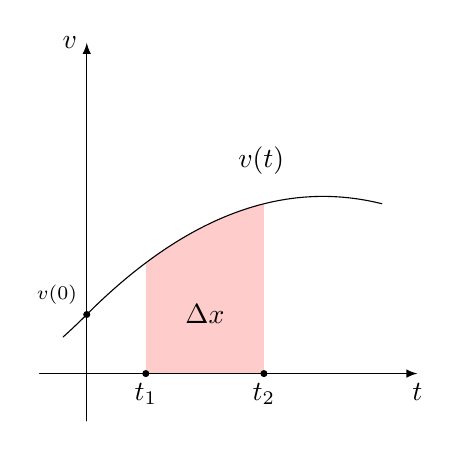
\begin{tikzpicture}
    [line cap=round,line join=round,x=2cm,y=2cm, scale=1.5, decoration={brace,amplitude=2pt}]
%main layer
%creating the ticks and xy-axis nodes
%some function
\fill[fill=red!20] (0.25,0) -- plot [domain=0.25:.75] (\x,{-\x^2/2+\x+0.25}) -- plot [domain=0.75: 0.25] (\x,0) -- cycle;

 \draw[smooth,samples=100,domain=-0.1:1.25]
                                 plot(\x,{-\x^2/2+\x+0.25});
 
  %\draw [darkgray,ultra thin] (0,0.479)-- (0.25,0.479);
  %\draw [darkgray,ultra thin] (0,0.938)-- (0.75,0.938);
 % \draw [darkgray,ultra thin] (0.25,0.479)-- (0.25,0.0);
  %\draw [darkgray,ultra thin] (0.75,0.938)-- (0.75,0);
%creating the curly braces with decorate
 
%  \draw [decorate,color=black!80!black] (0.25,0.0)--(0.75,0.0)
   %node [midway,anchor=north,inner sep=1pt, outer sep=1pt]{\small$\Delta x$};
    \fill[black] (0.25,0) circle (0.3mm) node [anchor=north ,scale=1] {$ t_1$};
     \fill[black] (0.75,0) circle (0.3mm) node [anchor=north ,scale=1] {$t_2$};
        \fill[black] (0,0.25) circle (0.3mm) node [anchor=south east,scale=1] {\scriptsize$ v(0)$};

  \draw[-latex,color=black,thin] (-0.2,0) -- (1.4,0) node [anchor=north ,scale=1] {$t$};
   \draw[-latex,color=black,thin] (0,-0.2) -- (0,1.4)node [anchor=east ,scale=1] {$v$};
    \draw (0.6,0.8) node [anchor=south west ,scale=1] {$v(t)$};
        \draw (0.5,0.25) node [anchor=center ,scale=1] {$\Delta x$};
        
 \end{tikzpicture}
 \hspace{1cm}
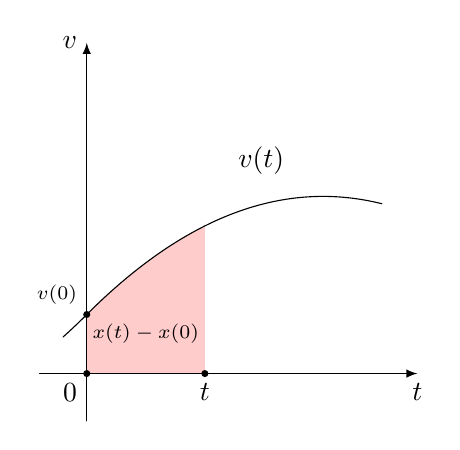
\begin{tikzpicture}
    [line cap=round,line join=round,x=2cm,y=2cm, scale=1.5, decoration={brace,amplitude=2pt}]
%main layer
%creating the ticks and xy-axis nodes
%some function
\fill[fill=red!20] (0,0) -- plot [domain=0:.5] (\x,{-\x^2/2+\x+0.25}) -- plot [domain=0.5: 0.0] (\x,0) -- cycle;

 \draw[smooth,samples=100,domain=-0.1:1.25]
                                 plot(\x,{-\x^2/2+\x+0.25});
 
  %\draw [darkgray,ultra thin] (0,0.479)-- (0.25,0.479);
  %\draw [darkgray,ultra thin] (0,0.938)-- (0.75,0.938);
 % \draw [darkgray,ultra thin] (0.25,0.479)-- (0.25,0.0);
  %\draw [darkgray,ultra thin] (0.75,0.938)-- (0.75,0);
%creating the curly braces with decorate
 
%  \draw [decorate,color=black!80!black] (0.25,0.0)--(0.75,0.0)
   %node [midway,anchor=north,inner sep=1pt, outer sep=1pt]{\small$\Delta x$};
    \fill[black] (0,0) circle (0.3mm) node [anchor=north east,scale=1] {$ 0$};
     \fill[black] (0.5,0) circle (0.3mm) node [anchor=north ,scale=1] {$t$};
      \fill[black] (0,0.25) circle (0.3mm) node [anchor=south east,scale=1] {\scriptsize$ v(0)$};

  \draw[-latex,color=black,thin] (-0.2,0) -- (1.4,0) node [anchor=north ,scale=1] {$t$};
   \draw[-latex,color=black,thin] (0,-0.2) -- (0,1.4)node [anchor=east ,scale=1] {$v$};
     \draw (0.6,0.8) node [anchor=south west ,scale=1] {$v(t)$};
        \draw (0.25,0.25) node [anchor=north ,scale=1] {\scriptsize$x(t)-x(0)$};
        
 \end{tikzpicture}
$$
\vspace{1cm}
$$
\begin{tikzpicture}
    [line cap=round,line join=round,x=2cm,y=2cm, scale=1.5, decoration={brace,amplitude=2pt}]
%main layer
%creating the ticks and xy-axis nodes
%some function
%\fill[fill=red!20] (0.25,0) -- plot [domain=0.25:.75] (\x,{-\x^3/6+\x^2/2+0.25\x+0.1}) -- plot [domain=0.75: 0.25] (\x,0) -- cycle;

 \draw[smooth,samples=100,domain=-0.1:1.25]
                                 plot(\x,{-\x^3/6+\x^2/2+\x/4+0.1});
 
  %\draw [darkgray,ultra thin] (0,0.479)-- (0.25,0.479);
  %\draw [darkgray,ultra thin] (0,0.938)-- (0.75,0.938);
 % \draw [darkgray,ultra thin] (0.25,0.479)-- (0.25,0.0);
  %\draw [darkgray,ultra thin] (0.75,0.938)-- (0.75,0);
%creating the curly braces with decorate
 
%  \draw [decorate,color=black!80!black] (0.25,0.0)--(0.75,0.0)
   %node [midway,anchor=north,inner sep=1pt, outer sep=1pt]{\small$\Delta x$};
           \fill[black] (0,0.1) circle (0.3mm) node [anchor=south east,scale=1] {\scriptsize$ x(0)$};

  \draw[-latex,color=black,thin] (-0.2,0) -- (1.4,0) node [anchor=north ,scale=1] {$t$};
   \draw[-latex,color=black,thin] (0,-0.2) -- (0,1.4)node [anchor=east ,scale=1] {$x$};
    \draw (0.6,0.8) node [anchor=south west ,scale=1] {$x(t)$};
              
 \end{tikzpicture}
 \hspace{1cm}
\begin{tikzpicture}
    [line cap=round,line join=round,x=2cm,y=2cm, scale=1.5, decoration={brace,amplitude=2pt}]
%main layer
%creating the ticks and xy-axis nodes
%some function
%\fill[fill=red!20] (0,0) -- plot [domain=0:.5] (\x,{-\x^2/2+\x+0.25}) -- plot [domain=0.5: 0.0] (\x,0) -- cycle;

 \draw[smooth,samples=100,domain=-0.1:1.25]
                                 plot(\x,{-\x^3/6+\x^2/2+\x/4+0.1});

 
  %\draw [darkgray,ultra thin] (0,0.479)-- (0.25,0.479);
  %\draw [darkgray,ultra thin] (0,0.938)-- (0.75,0.938);
 % \draw [darkgray,ultra thin] (0.25,0.479)-- (0.25,0.0);
  %\draw [darkgray,ultra thin] (0.75,0.938)-- (0.75,0);
%creating the curly braces with decorate
 
%  \draw [decorate,color=black!80!black] (0.25,0.0)--(0.75,0.0)
   %node [midway,anchor=north,inner sep=1pt, outer sep=1pt]{\small$\Delta x$};
  
      \fill[black] (0,0.1) circle (0.3mm) node [anchor=south east,scale=1] {\scriptsize$ x(0)$};

  \draw[-latex,color=black,thin] (-0.2,0) -- (1.4,0) node [anchor=north ,scale=1] {$t$};
   \draw[-latex,color=black,thin] (0,-0.2) -- (0,1.4)node [anchor=east ,scale=1] {$x$};
     \draw (0.6,0.8) node [anchor=south west ,scale=1] {$x(t)$};
       % \draw (0.25,0.25) node [anchor=center ,scale=1] {\scriptsize$x(t)-x(0)$};
        
 \end{tikzpicture}
$$
\newpage

\section{Simple 1-D Motion}
\subsection{Constant Velocity}
\marginnote[50pt]{The situation of constant velocity means it is not changing or its rate of change is zero.  Constant velocity is zero acceleration.  Zero acceleration yields no area under the curve.  $\Delta v=0$ }
\marginnote[190pt]{Since the velocity doesn't change $\Delta v=0$ and the velocity stays as $v_0$, all day everyday. }
\marginnote[160pt]{If the velocity is constant the slope of $x(t)$ is constant.   It is a straight line with a slope $v_0$ and vertical intercept of $x_0$ . The curvature is zero. }
\begin{center}
\begin{tabular}{cc}
\begin{minipage}{5cm}
$$a(t)=\text{Slope}(v(t))=0$$
%$$\bar{a}=0$$
$$\Delta v=\text{Area under }a(t)=0$$
%$$\Delta v=\bar{a}\Delta t=0$$
$$v(t)=v(0)+\Delta v$$
$$v(t)=v(0)$$
\end{minipage}
&
\begin{minipage}{5cm}
$$\begin{tikzpicture}
    [line cap=round,line join=round,x=2cm,y=2cm, scale=1.5, decoration={brace,amplitude=2pt}]
%main layer
%creating the ticks and xy-axis nodes
%some function

 
  %\draw [darkgray,ultra thin] (0,0.479)-- (0.25,0.479);
  %\draw [darkgray,ultra thin] (0,0.938)-- (0.75,0.938);
 % \draw [darkgray,ultra thin] (0.25,0.479)-- (0.25,0.0);
  %\draw [darkgray,ultra thin] (0.75,0.938)-- (0.75,0);
%creating the curly braces with decorate
 
%  \draw [decorate,color=black!80!black] (0.25,0.0)--(0.75,0.0)
   %node [midway,anchor=north,inner sep=1pt, outer sep=1pt]{\small$\Delta x$};
   

  \draw[-latex,color=black,thin] (-0.2,0) -- (1.4,0) node [anchor=north ,scale=1] {$t$};
   \draw[-latex,color=black,thin] (0,-0.2) -- (0,1.4)node [anchor=east ,scale=1] {$a$};
    \draw (0.6,0.6) node [anchor=south west ,scale=1] {\scriptsize$a(t)=0$};
      %  \draw (0.25,0.3) node [anchor=west ,scale=1] {\scriptsize$v(t)-v(0)=\int a(t)dt=0$};
        
 \end{tikzpicture}$$
 \end{minipage}
 \end{tabular}
 \end{center}
 
 \vspace{1cm}
 \begin{center}
\begin{tabular}{cc}
\begin{minipage}{5cm}
$$v(t)=v(0)=v_0=\text{constant}$$
$$v(t)=\text{Slope}(x(t))$$
$$\Delta x=\text{Area under }v(t)$$
$$\Delta x=v_0 \Delta t$$
$$x(t)=x(0)+v_0 t$$

\end{minipage}
&
\begin{minipage}{5cm}
$$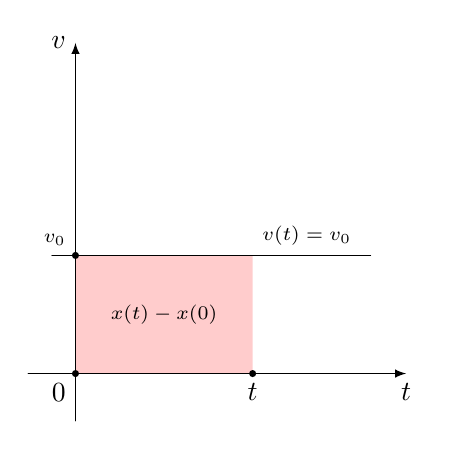
\begin{tikzpicture}
    [line cap=round,line join=round,x=2cm,y=2cm, scale=1.5, decoration={brace,amplitude=2pt}]
%main layer
%creating the ticks and xy-axis nodes
%some function
\fill[fill=red!20] (0,0) -- plot [domain=0:.75] (\x,0.5) -- plot [domain=0.75: 0.0] (\x,0) -- cycle;

 \draw[smooth,samples=100,domain=-0.1:1.25]
                                 plot(\x,0.5);
 
  %\draw [darkgray,ultra thin] (0,0.479)-- (0.25,0.479);
  %\draw [darkgray,ultra thin] (0,0.938)-- (0.75,0.938);
 % \draw [darkgray,ultra thin] (0.25,0.479)-- (0.25,0.0);
  %\draw [darkgray,ultra thin] (0.75,0.938)-- (0.75,0);
%creating the curly braces with decorate
 
%  \draw [decorate,color=black!80!black] (0.25,0.0)--(0.75,0.0)
   %node [midway,anchor=north,inner sep=1pt, outer sep=1pt]{\small$\Delta x$};
    \fill[black] (0,0) circle (0.3mm) node [anchor=north east,scale=1] {$ 0$};
     \fill[black] (0.75,0) circle (0.3mm) node [anchor=north ,scale=1] {$t$};
      \fill[black] (0,0.5) circle (0.3mm) node [anchor=south east,scale=1] {\scriptsize$ v_0$};

  \draw[-latex,color=black,thin] (-0.2,0) -- (1.4,0) node [anchor=north ,scale=1] {$t$};
   \draw[-latex,color=black,thin] (0,-0.2) -- (0,1.4)node [anchor=east ,scale=1] {$v$};
     \draw (0.75,0.5) node [anchor=south west ,scale=1] {\scriptsize$v(t)=v_0$};
        \draw (0.375,0.25) node [anchor=center ,scale=1] {\scriptsize$x(t)-x(0)$};
        
 \end{tikzpicture}
$$

  \end{minipage}
 \end{tabular}
 \end{center}
 

 \vspace{1cm}
 \begin{center}
\begin{tabular}{cc}
\begin{minipage}{5cm}
 

$$x(t)=x_0+v_0t$$

\end{minipage}
&
\begin{minipage}{5cm}

$$\begin{tikzpicture}
    [line cap=round,line join=round,x=2cm,y=2cm, scale=1.5, decoration={brace,amplitude=2pt}]
%main layer
%creating the ticks and xy-axis nodes
%some function
%\fill[fill=red!20] (0,0) -- plot [domain=0:.5] (\x,{-\x^2/2+\x+0.25}) -- plot [domain=0.5: 0.0] (\x,0) -- cycle;

 \draw[smooth,samples=100,domain=-0.1:1.25]
                                 plot(\x,{0.25+\x/2});

 
  %\draw [darkgray,ultra thin] (0,0.479)-- (0.25,0.479);
  %\draw [darkgray,ultra thin] (0,0.938)-- (0.75,0.938);
 % \draw [darkgray,ultra thin] (0.25,0.479)-- (0.25,0.0);
  %\draw [darkgray,ultra thin] (0.75,0.938)-- (0.75,0);
%creating the curly braces with decorate
 
%  \draw [decorate,color=black!80!black] (0.25,0.0)--(0.75,0.0)
   %node [midway,anchor=north,inner sep=1pt, outer sep=1pt]{\small$\Delta x$};
  
      \fill[black] (0,0.25) circle (0.3mm) node [anchor=south east,scale=1] {\scriptsize$ x_0$};

  \draw[-latex,color=black,thin] (-0.2,0) -- (1.4,0) node [anchor=north ,scale=1] {$t$};
   \draw[-latex,color=black,thin] (0,-0.2) -- (0,1.4)node [anchor=east ,scale=1] {$x$};
     \draw (0.75,0.9) node [anchor=center ,scale=1] {\scriptsize$x(t)=x_0+v_0t$};
       % \draw (0.25,0.25) node [anchor=center ,scale=1] {\scriptsize$x(t)-x(0)$};
        
 \end{tikzpicture}
$$
 \end{minipage}
 \end{tabular}
 \end{center}
\newpage
\subsection{Constant Acceleration}
\marginnote[50pt]{Constant acceleration is smooth, zero jerk.  It generates a rectangular area beneath it representing the change in velocity.  $\text{Area}=\text{height}\times\text{base}$ so $\Delta v= a t$.  The acceleration is the average acceleration because it dent change.  It stays constant $a$ all day everyday. }
\marginnote[150pt]{Since the acceleration is constant the slope of the velocity versus time graph is constant.  $v(t)$ is a straight line with slope a. The vertical intercept is $v_0$.  The area underneath the function is the displacement.  It may be computed using the triangular portion $\nicefrac{at^2}{2}$ and rectangular portion $v_0t$. }
\marginnote[160pt]{The slope of $x(t)$ is changing linearly so $x(t)$ is parabolic.   It is a quadratic function with vertical intercept of $x_0$. }
\begin{center}
\begin{tabular}{cc}
\begin{minipage}{5cm}
$$\text{Slope}(a(t))=0$$
$$a(t)=a=\text{constant}$$
$$\Delta v=\text{Area under }a(t)$$
$$\Delta v=at$$
$$v(t)=v(0)+\Delta v$$
$$v(t)=v(0)+at$$

\end{minipage}
&
\begin{minipage}{5cm}
$$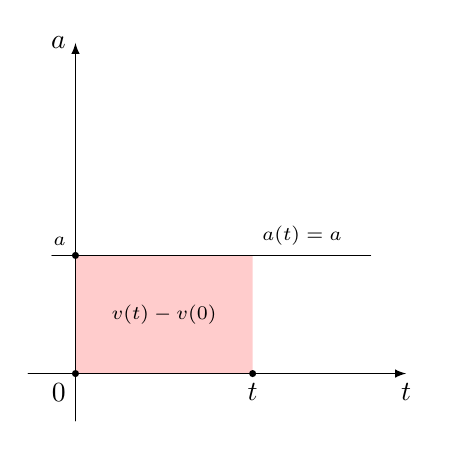
\begin{tikzpicture}
    [line cap=round,line join=round,x=2cm,y=2cm, scale=1.5, decoration={brace,amplitude=2pt}]
%main layer
%creating the ticks and xy-axis nodes
%some function
\fill[fill=red!20] (0,0) -- plot [domain=0:.75] (\x,0.5) -- plot [domain=0.75: 0.0] (\x,0) -- cycle;

 \draw[smooth,samples=100,domain=-0.1:1.25]
                                 plot(\x,0.5);
 
  %\draw [darkgray,ultra thin] (0,0.479)-- (0.25,0.479);
  %\draw [darkgray,ultra thin] (0,0.938)-- (0.75,0.938);
 % \draw [darkgray,ultra thin] (0.25,0.479)-- (0.25,0.0);
  %\draw [darkgray,ultra thin] (0.75,0.938)-- (0.75,0);
%creating the curly braces with decorate
 
%  \draw [decorate,color=black!80!black] (0.25,0.0)--(0.75,0.0)
   %node [midway,anchor=north,inner sep=1pt, outer sep=1pt]{\small$\Delta x$};
    \fill[black] (0,0) circle (0.3mm) node [anchor=north east,scale=1] {$ 0$};
     \fill[black] (0.75,0) circle (0.3mm) node [anchor=north ,scale=1] {$t$};
      \fill[black] (0,0.5) circle (0.3mm) node [anchor=south east,scale=1] {\scriptsize$ a$};

  \draw[-latex,color=black,thin] (-0.2,0) -- (1.4,0) node [anchor=north ,scale=1] {$t$};
   \draw[-latex,color=black,thin] (0,-0.2) -- (0,1.4)node [anchor=east ,scale=1] {$a$};
     \draw (0.75,0.5) node [anchor=south west ,scale=1] {\scriptsize$a(t)=a$};
        \draw (0.375,0.25) node [anchor=center ,scale=1] {\scriptsize$v(t)-v(0)$};
        
 \end{tikzpicture}
$$

 \end{minipage}
 \end{tabular}
 \end{center}
 
 \vspace{1cm}
 \begin{center}
\begin{tabular}{cc}
\begin{minipage}{5cm}
$$v(t)=v_0+at$$
$$v(t)=\text{Slope}(x(t))$$
$$\Delta x=\text{Area under }v(t)$$
$$\Delta x =v_0t+\frac{1}{2}at^2$$
$$x(t)=x(0)+\Delta x$$
$$x(t)=x(0)+v_0t+\frac{1}{2}at^2$$
\end{minipage}
&
\begin{minipage}{5cm}
$$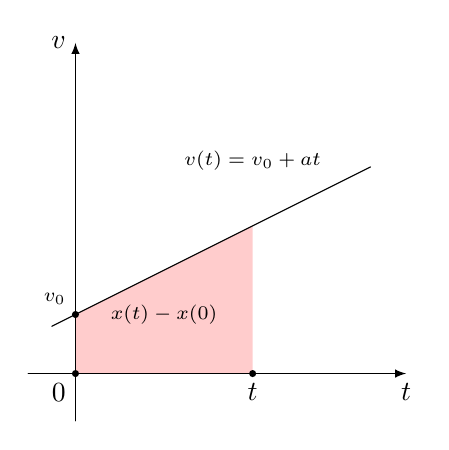
\begin{tikzpicture}
    [line cap=round,line join=round,x=2cm,y=2cm, scale=1.5, decoration={brace,amplitude=2pt}]
%main layer
%creating the ticks and xy-axis nodes
%some function
\fill[fill=red!20] (0,0) -- plot [domain=0:.75] (\x,{\x/2+0.25}) -- plot [domain=0.75: 0.0] (\x,0) -- cycle;

 \draw[smooth,samples=100,domain=-0.1:1.25]
                                 plot(\x,{\x/2+0.25});
 
  %\draw [darkgray,ultra thin] (0,0.479)-- (0.25,0.479);
  %\draw [darkgray,ultra thin] (0,0.938)-- (0.75,0.938);
 % \draw [darkgray,ultra thin] (0.25,0.479)-- (0.25,0.0);
  %\draw [darkgray,ultra thin] (0.75,0.938)-- (0.75,0);
%creating the curly braces with decorate
 
%  \draw [decorate,color=black!80!black] (0.25,0.0)--(0.75,0.0)
   %node [midway,anchor=north,inner sep=1pt, outer sep=1pt]{\small$\Delta x$};
    \fill[black] (0,0) circle (0.3mm) node [anchor=north east,scale=1] {$ 0$};
     \fill[black] (0.75,0) circle (0.3mm) node [anchor=north ,scale=1] {$t$};
      \fill[black] (0,0.25) circle (0.3mm) node [anchor=south east,scale=1] {\scriptsize$ v_0$};

  \draw[-latex,color=black,thin] (-0.2,0) -- (1.4,0) node [anchor=north ,scale=1] {$t$};
   \draw[-latex,color=black,thin] (0,-0.2) -- (0,1.4)node [anchor=east ,scale=1] {$v$};
     \draw (0.75,0.9) node [anchor=center ,scale=1] {\scriptsize$v(t)=v_0+at$};
        \draw (0.375,0.25) node [anchor=center ,scale=1] {\scriptsize$x(t)-x(0)$};
        
 \end{tikzpicture}
$$

  \end{minipage}
 \end{tabular}
 \end{center}
 

 \vspace{1cm}
 \begin{center}
\begin{tabular}{cc}
\begin{minipage}{5cm}
 
$$x(t)=x_0+v_0t+\frac{at^2}{2}$$

\end{minipage}
&
\begin{minipage}{5cm}

$$\begin{tikzpicture}
    [line cap=round,line join=round,x=2cm,y=2cm, scale=1.5, decoration={brace,amplitude=2pt}]
%main layer
%creating the ticks and xy-axis nodes
%some function
%\fill[fill=red!20] (0,0) -- plot [domain=0:.5] (\x,{-\x^2/2+\x+0.25}) -- plot [domain=0.5: 0.0] (\x,0) -- cycle;

 \draw[smooth,samples=100,domain=-0.1:1.25]
                                 plot(\x,{0.25+\x/4+\x^2/2});

 
  %\draw [darkgray,ultra thin] (0,0.479)-- (0.25,0.479);
  %\draw [darkgray,ultra thin] (0,0.938)-- (0.75,0.938);
 % \draw [darkgray,ultra thin] (0.25,0.479)-- (0.25,0.0);
  %\draw [darkgray,ultra thin] (0.75,0.938)-- (0.75,0);
%creating the curly braces with decorate
 
%  \draw [decorate,color=black!80!black] (0.25,0.0)--(0.75,0.0)
   %node [midway,anchor=north,inner sep=1pt, outer sep=1pt]{\small$\Delta x$};
  
      \fill[black] (0,0.25) circle (0.3mm) node [anchor=south east,scale=1] {\scriptsize$ x_0$};

  \draw[-latex,color=black,thin] (-0.2,0) -- (1.4,0) node [anchor=north ,scale=1] {$t$};
   \draw[-latex,color=black,thin] (0,-0.2) -- (0,1.4)node [anchor=east ,scale=1] {$x$};
     \draw (0.6,0.6) node [anchor=north west ,scale=1] {\scriptsize$x(t)=x_0+v_0t+\frac{at^2}{2}$};
       % \draw (0.25,0.25) node [anchor=center ,scale=1] {\scriptsize$x(t)-x(0)$};
        
 \end{tikzpicture}
$$
 \end{minipage}
 \end{tabular}
 \end{center}
\newpage
\
\subsubsection{Removing Time Dependence}
\vspace{1cm}
\marginnote[50pt]{Removing time dependence is to take the function $v(t)$ and determine $v(x)$.  To determine the velocity of an object dependent on its position in space.}
\marginnote[150pt]{Graphically this corresponds to a linear graph with vertical axis $v^2$ and horizontal axis $x$.  }
\marginnote[160pt]{Reversing this procedure is accomplished by determining $\Delta t$ as the area beneath the function $\nicefrac{1}{v(x)}$ graphed versus $x$. }
$$v=v_0+at \ \ \Longrightarrow \ \ t=\frac{v-v_0}{a}$$
$$x=x_0+v_0t+\frac{at^2}{2}=x_0+v_0(\frac{v-v_0}{a})+\frac{a(\frac{v-v_0}{a})^2}{2}=x_0+\frac{v^2-v^2_0}{2a} $$
$$v^2-v_0^2=2a(x-x_0)$$
\vspace{1cm}
$$\begin{tikzpicture}
    [line cap=round,line join=round,x=2cm,y=2cm, scale=1.5, decoration={brace,amplitude=2pt}]
%main layer
%creating the ticks and xy-axis nodes
%some function
%\fill[fill=red!20] (0,0) -- plot [domain=0:.5] (\x,{-\x^2/2+\x+0.25}) -- plot [domain=0.5: 0.0] (\x,0) -- cycle;

 \draw[smooth,samples=100,domain=-0.1:1.25]
                                 plot(\x,{\x});

 
  %\draw [darkgray,ultra thin] (0,0.479)-- (0.25,0.479);
  %\draw [darkgray,ultra thin] (0,0.938)-- (0.75,0.938);
 % \draw [darkgray,ultra thin] (0.25,0.479)-- (0.25,0.0);
  %\draw [darkgray,ultra thin] (0.75,0.938)-- (0.75,0);
%creating the curly braces with decorate
 
%  \draw [decorate,color=black!80!black] (0.25,0.0)--(0.75,0.0)
   %node [midway,anchor=north,inner sep=1pt, outer sep=1pt]{\small$\Delta x$};
  
      \fill[black] (0,0) circle (0.3mm) node [anchor=south east,scale=1] {\scriptsize$ v^2_0$};
       \fill[black] (0,0) circle (0.3mm) node [anchor=north west,scale=1] {\scriptsize$ x_0$};

  \draw[-latex,color=black,thin] (-0.2,0) -- (1.4,0) node [anchor=north ,scale=1] {$x$};
   \draw[-latex,color=black,thin] (0,-0.2) -- (0,1.4)node [anchor=east ,scale=1] {$v^2$};
     \draw (0.4,0.5) node [anchor=north west ,scale=1] {\scriptsize$v^2-v_0^2=\overbrace{2a}^{\textit{slope}}(x-x_0)$};
       % \draw (0.25,0.25) node [anchor=center ,scale=1] {\scriptsize$x(t)-x(0)$};
        
 \end{tikzpicture}
$$
\vspace{1cm}
%$$\Delta v^2=2\int a(x)\ dx\ \longrightarrow \ \Delta v^2=2\int \overrightarrow{a}(\overrightarrow{\scriptr})\cdot d\overrightarrow{\scriptr}\ \longrightarrow \ v(x) $$
\vspace{1cm}
\subsubsection{Returning Time Dependence}
\vspace{1cm}
$$\{v(x),\Delta x\}\longrightarrow t(x) \longrightarrow x(t)$$
\vspace{1cm}
$$\Delta t=\text{Area under }\frac{1}{v(x)}$$


\subsection{Equations of Simple 1-D Translational Motion}
\vspace{1cm}
\marginnote[50pt]{These are the kinematic equations of motion for a system of constant acceleration}
\marginnote[150pt]{Near the surface of the earth the acceleration due to gravity is fairly constant.  Under a constant acceleration toward the ground.  If up is taken as positive the acceleration is a negative constant.}
\marginnote[150pt]{Graphically this corresponds to a linear $v(t)$ function with a slope of $-g$ and a downwardly concave parabolic $x(t)$ function.  }

\begin{center}
\begin{tabular}{cc}
\begin{minipage}{6cm}
\subsubsection{Constant Velocity}
$$v=v_0$$

$$x=x_0+vt$$
\vspace{0.75cm}
\end{minipage}
&
\begin{minipage}{6cm}
\subsubsection{Constant Acceleration}
$$v=v_0+at$$
$$\bar{v}=\frac{v_0+v}{2}$$
$$x=x_0+v_0t+\frac{at^2}{2}=x_0+\bar{v}t$$
$$v^2-v_0^2=2a(x-x_0)$$

 \end{minipage}
 \end{tabular}
 \end{center}
 
 
 \subsection{Gravity at Earth's Surface}
 \vspace{1cm}
 $$a=-g=-9.81\frac{\text{m}}{\text{s}^2}$$
 
 $$v=v_0-gt$$

$$x=x_0+v_0t-\frac{gt^2}{2}$$

$$v^2-v_0^2=-2g(x-x_0)$$
\vspace{1cm}
$$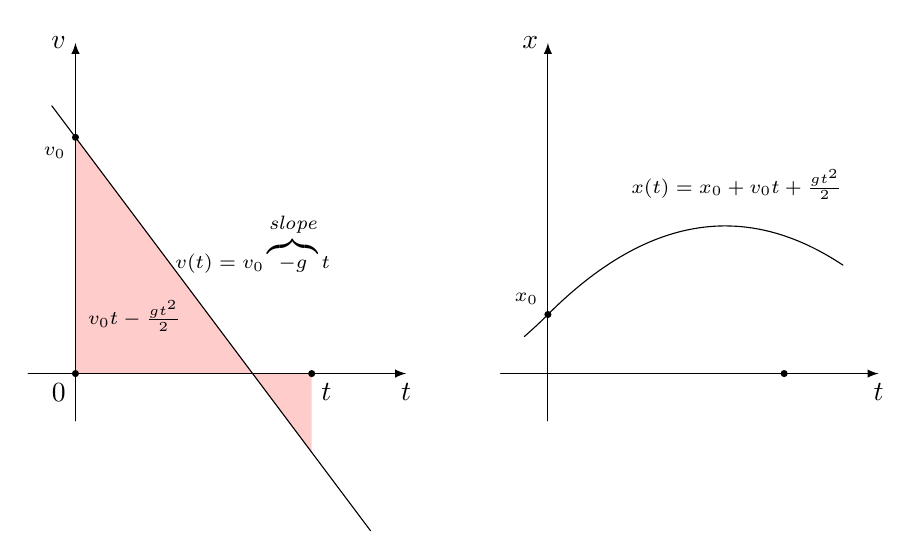
\begin{tikzpicture}
    [line cap=round,line join=round,x=2cm,y=2cm, scale=1.5, decoration={brace,amplitude=2pt}]
%main layer
%creating the ticks and xy-axis nodes
%some function
\fill[fill=red!20] (0,0) -- plot [domain=0:1] (\x,{-\x/0.75+1}) -- plot [domain=01: 0.0] (\x,0) -- cycle;

 \draw[smooth,samples=100,domain=-0.1:1.25]
                                 plot(\x,{-\x/0.75+1});
 
  %\draw [darkgray,ultra thin] (0,0.479)-- (0.25,0.479);
  %\draw [darkgray,ultra thin] (0,0.938)-- (0.75,0.938);
 % \draw [darkgray,ultra thin] (0.25,0.479)-- (0.25,0.0);
  %\draw [darkgray,ultra thin] (0.75,0.938)-- (0.75,0);
%creating the curly braces with decorate
 
%  \draw [decorate,color=black!80!black] (0.25,0.0)--(0.75,0.0)
   %node [midway,anchor=north,inner sep=1pt, outer sep=1pt]{\small$\Delta x$};
    \fill[black] (0,0) circle (0.3mm) node [anchor=north east,scale=1] {$ 0$};
     \fill[black] (1,0) circle (0.3mm) node [anchor=north west ,scale=1] {$t$};
      \fill[black] (0,1) circle (0.3mm) node [anchor=north east,scale=1] {\scriptsize$ v_0$};

  \draw[-latex,color=black,thin] (-0.2,0) -- (1.4,0) node [anchor=north ,scale=1] {$t$};
   \draw[-latex,color=black,thin] (0,-0.2) -- (0,1.4)node [anchor=east ,scale=1] {$v$};
     \draw (0.75,0.55) node [anchor=center ,scale=1] {\scriptsize$v(t)=v_0\overbrace{-g}^{\textit{slope}}t$};
        \draw (0.25,0.35) node [anchor=north ,scale=1] {\scriptsize$v_0t-\frac{gt^2}{2}$};
        
        
        \begin{scope}[shift={(2,0)}]
 \draw[smooth,samples=100,domain=-0.1:1.25]
                                 plot(\x,{0.25-\x^2/1.5+\x});
      \fill[black] (0,0.25) circle (0.3mm) node [anchor=south east,scale=1] {\scriptsize$ x_0$};

  \draw[-latex,color=black,thin] (-0.2,0) -- (1.4,0) node [anchor=north ,scale=1] {$t$};
   \draw[-latex,color=black,thin] (0,-0.2) -- (0,1.4)node [anchor=east ,scale=1] {$x$};
     \draw (0.8,0.8) node [anchor=center ,scale=1] {\scriptsize$x(t)=x_0+v_0t+\frac{gt^2}{2}$};
     \fill[black] (1,0) circle (0.3mm) node [anchor=north west ,scale=1] {$$};
\end{scope}
 \end{tikzpicture}
$$
\newpage
 \section{2-D Constant Velocity}
 \marginnote[50pt]{In two dimensions position, velocity and acceleration are represented by 2D vectors.  Acceleration is zero so velocity does not change from its initial state $\overrightarrow{v}_0$.}
 
 \marginnote[300pt]{The velocity vector does not change.  The position vector propagates linearly in the $\hat{v}$ direction from the initial position $\overrightarrow{r}_0$..}
 \vspace{1cm}
 $$\overrightarrow{a}=0$$
 \vspace{1cm}
$$v_x=v_{0x}$$
$$v_y=v_{0y}$$
$$\overrightarrow{v}=\left(\begin{array}{c} v_x \\ v_y \end{array}\right)=\left(\begin{array}{c} v_{0x} \\ v_{0y} \end{array}\right)=\overrightarrow{v}_0$$
\vspace{1cm}
$$x=x_0+v_{0x}t$$
$$y=y_0+v_{0y}t$$

$$\overrightarrow{r}=\left(\begin{array}{c} x \\ y \end{array}\right)=\left(\begin{array}{c} x_0+v_{0x}t \\ y_0+v_{0y}t \end{array}\right)=\left(\begin{array}{c} x_0 \\ y_0 \end{array}\right)+\left(\begin{array}{c}v_{0x} \\ v_{0y} \end{array}\right)t=\overrightarrow{r}_0+\overrightarrow{v}_0t$$

\vspace{1cm}$$
 \begin{tikzpicture}
    [line cap=round,line join=round,x=2cm,y=2cm, scale=1.5, decoration={brace,amplitude=2pt}]
%main layer
%creating the ticks and xy-axis nodes
%some function
%\fill[fill=red!20] (0,0) -- plot [domain=0:1] (\x,{-\x/0.75+1}) -- plot [domain=01: 0.0] (\x,0) -- cycle;

% \draw[smooth,samples=1000,domain=-0.1:1.25]
     %                            plot(\x,{-\x/0.75+1});
 
  %\draw [darkgray,ultra thin] (0,0.479)-- (0.25,0.479);
  %\draw [darkgray,ultra thin] (0,0.938)-- (0.75,0.938);
 % \draw [darkgray,ultra thin] (0.25,0.479)-- (0.25,0.0);
  %\draw [darkgray,ultra thin] (0.75,0.938)-- (0.75,0);
%creating the curly braces with decorate
 
%  \draw [decorate,color=black!80!black] (0.25,0.0)--(0.75,0.0)
   %node [midway,anchor=north,inner sep=1pt, outer sep=1pt]{\small$\Delta x$};
   % \fill[black] (0,0) circle (0.3mm) node [anchor=north east,scale=1] {$ 0$};
   %  \fill[black] (1,0) circle (0.3mm) node [anchor=north west ,scale=1] {$t$};
      \fill[black] (0.6,0.3) circle (0.3mm) node [anchor=south east,scale=1] {\scriptsize$\overrightarrow{v}=\overrightarrow{v}_0$};

 % \draw[-latex,color=black,thin] (-0.1,0.15) -- (1.2,0.8);
   \draw[-latex,color=black,thin] (0,-0.2) -- (0,1.4)node [anchor=east ,scale=1] {$v_y$};
    \draw[-stealth,color=black,thin] (-0.2,0) -- (1.4,0) node [anchor=north ,scale=1] {$v_x$};
    % \draw (0.75,0.8) node [anchor=center ,scale=1] {\scriptsize$\overrightarrow{r}(t)=\overrightarrow{r}_0+\overrightarrow{v}t$};
      %  \draw (0.25,0.35) node [anchor=north ,scale=1] {\scriptsize$v_0t-\frac{gt^2}{2}$};
        
        

 \end{tikzpicture}
 \hspace{1cm}
 \begin{tikzpicture}
    [line cap=round,line join=round,x=2cm,y=2cm, scale=1.5, decoration={brace,amplitude=2pt}]
%main layer
%creating the ticks and xy-axis nodes
%some function
%\fill[fill=red!20] (0,0) -- plot [domain=0:1] (\x,{-\x/0.75+1}) -- plot [domain=01: 0.0] (\x,0) -- cycle;

% \draw[smooth,samples=1000,domain=-0.1:1.25]
     %                            plot(\x,{-\x/0.75+1});
 
  %\draw [darkgray,ultra thin] (0,0.479)-- (0.25,0.479);
  %\draw [darkgray,ultra thin] (0,0.938)-- (0.75,0.938);
 % \draw [darkgray,ultra thin] (0.25,0.479)-- (0.25,0.0);
  %\draw [darkgray,ultra thin] (0.75,0.938)-- (0.75,0);
%creating the curly braces with decorate
 
%  \draw [decorate,color=black!80!black] (0.25,0.0)--(0.75,0.0)
   %node [midway,anchor=north,inner sep=1pt, outer sep=1pt]{\small$\Delta x$};
   % \fill[black] (0,0) circle (0.3mm) node [anchor=north east,scale=1] {$ 0$};
   %  \fill[black] (1,0) circle (0.3mm) node [anchor=north west ,scale=1] {$t$};
      \fill[black] (0.3,0.35) circle (0.3mm) node [anchor=south east,scale=1] {\scriptsize$\overrightarrow{r}_0$};

  \draw[-latex,color=black,thin] (-0.1,0.15) -- (1.2,0.8);
   \draw[-latex,color=black,thin] (0,-0.2) -- (0,1.4)node [anchor=east ,scale=1] {$y$};
    \draw[-stealth,color=black,thin] (-0.2,0) -- (1.4,0) node [anchor=north ,scale=1] {$x$};
     \draw (0.75,0.8) node [anchor=center ,scale=1] {\scriptsize$\overrightarrow{r}(t)=\overrightarrow{r}_0+\overrightarrow{v}_0t$};
      %  \draw (0.25,0.35) node [anchor=north ,scale=1] {\scriptsize$v_0t-\frac{gt^2}{2}$};
        
        

 \end{tikzpicture}
$$
\vspace{1cm}
\newpage

\section{Projectile Motion}
\marginnote[0pt]{In projectile motion there is no acceleration in the horizontal direction and constant acceleration in the vertical direction.  Under these conditions the initial position and velocity completely determines the evolution of the system.  Take x and y as the horizontal and vertical components respectively.  In the $x$ direction there is no acceleration and constant velocity making $x(t)$ a linear function.  In the $y$ direction the acceleration is constant and velocity changing linearly as a function of time.  This makes $y(t)$ a parabolic function.  The trajectory is also a parabolic function.}
$$\overrightarrow{a}=-g\hat{y}=\left(\begin{array}{c} 0 \\ -g \end{array}\right)$$
$$v_x=v_{0x}$$
$$v_y=v_{0y}+a_yt=v_{0y}-gt$$
$$\overrightarrow{v}=\left(\begin{array}{c} v_x \\ v_y \end{array}\right)=\left(\begin{array}{c} v_{0x} \\ v_{0y}-gt \end{array}\right)=\left(\begin{array}{c} v_{0x} \\ v_{0y} \end{array}\right)+\left(\begin{array}{c}0 \\ -g \end{array}\right)t=\overrightarrow{v}_0+\overrightarrow{a}t$$
$$x=x_0+v_{0x}t$$
$$y=y_0+v_{0y}t-\frac{gt^2}{2}$$
$$\overrightarrow{r}=\left(\begin{array}{c} x \\ y \end{array}\right)=\left(\begin{array}{c} x_0+v_{0x}t \\ y_0+v_{0y}t -\frac{gt^2}{2}\end{array}\right)=\left(\begin{array}{c} x_0 \\ y_0 \end{array}\right)+\left(\begin{array}{c}v_{0x} \\ v_{0y} \end{array}\right)t+\left(\begin{array}{c} 0 \\ -g \end{array}\right)\frac{t^2}{2}=\overrightarrow{r}_0+\overrightarrow{v}_0t+\overrightarrow{a}\frac{t^2}{2}$$

$$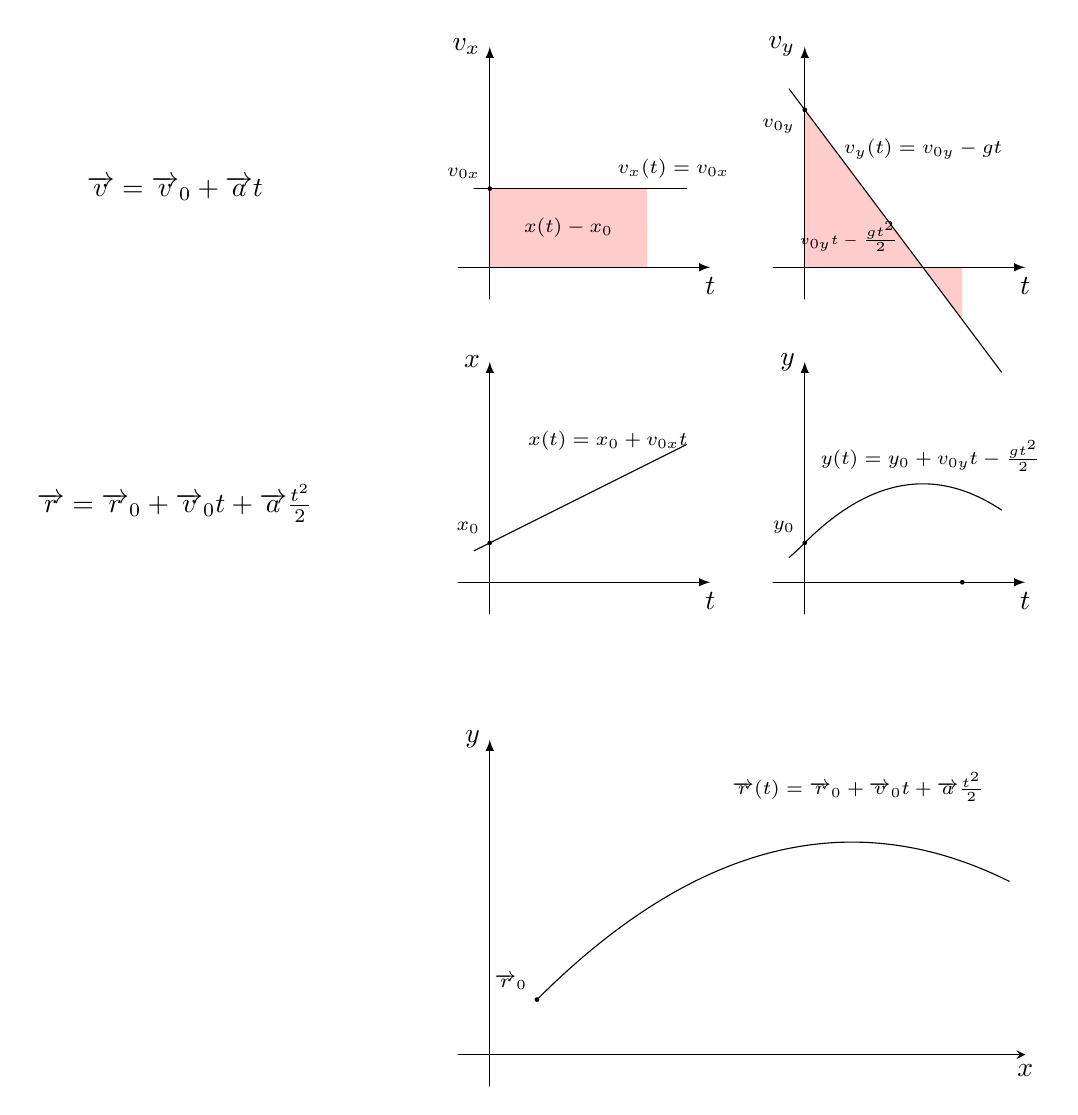
\begin{tikzpicture}
    [line cap=round,line join=round,x=2cm,y=2cm, scale=1, decoration={brace,amplitude=2pt}]
%main layer
%creating the ticks and xy-axis nodes
%some function
\fill[fill=red!20] (0,0) -- plot [domain=0:1] (\x,{-\x/0.75+1}) -- plot [domain=01: 0.0] (\x,0) -- cycle;

 \draw[smooth,samples=100,domain=-0.1:1.25]
                                 plot(\x,{-\x/0.75+1});
 
  %\draw [darkgray,ultra thin] (0,0.479)-- (0.25,0.479);
  %\draw [darkgray,ultra thin] (0,0.938)-- (0.75,0.938);
 % \draw [darkgray,ultra thin] (0.25,0.479)-- (0.25,0.0);
  %\draw [darkgray,ultra thin] (0.75,0.938)-- (0.75,0);
%creating the curly braces with decorate
 
%  \draw [decorate,color=black!80!black] (0.25,0.0)--(0.75,0.0)
   %node [midway,anchor=north,inner sep=1pt, outer sep=1pt]{\small$\Delta x$};
    %\fill[black] (0,0) circle (0.3mm) node [anchor=north east,scale=1] {$ 0$};
    % \fill[black] (1,0) circle (0.3mm) node [anchor=north west ,scale=1] {$t$};
      \fill[black] (0,1) circle (0.3mm) node [anchor=north east,scale=1] {\scriptsize$ v_{0y}$};

  \draw[-latex,color=black,thin] (-0.2,0) -- (1.4,0) node [anchor=north ,scale=1] {$t$};
   \draw[-latex,color=black,thin] (0,-0.2) -- (0,1.4)node [anchor=east ,scale=1] {$v_y$};
     \draw (0.75,0.75) node [anchor=center ,scale=1] {\scriptsize$v_y(t)=v_{0y}-gt$};
        \draw (0.28,0.35) node [anchor=north ,scale=1] {\tiny$v_{0y}t-\frac{gt^2}{2}$};
        
        
        \begin{scope}[shift={(0,-2)}]
 \draw[smooth,samples=100,domain=-0.1:1.25]
                                 plot(\x,{0.25-\x^2/1.5+\x});
      \fill[black] (0,0.25) circle (0.3mm) node [anchor=south east,scale=1] {\scriptsize$ y_0$};

  \draw[-latex,color=black,thin] (-0.2,0) -- (1.4,0) node [anchor=north ,scale=1] {$t$};
   \draw[-latex,color=black,thin] (0,-0.2) -- (0,1.4)node [anchor=east ,scale=1] {$y$};
     \draw (0.8,0.8) node [anchor=center ,scale=1] {\scriptsize$y(t)=y_0+v_{0y}t-\frac{gt^2}{2}$};
     \fill[black] (1,0) circle (0.3mm) node [anchor=north west ,scale=1] {$$};
\end{scope}

\begin{scope}[shift={(-2,0)}]
\fill[fill=red!20] (0,0) -- plot [domain=0:1] (\x,0.5) -- plot [domain=1: 0.0] (\x,0) -- cycle;

 \draw[smooth,samples=100,domain=-0.1:1.25]
                                 plot(\x,0.5);

  %  \fill[black] (0,0) circle (0.3mm) node [anchor=north east,scale=1] {$ 0$};
    % \fill[black] (0.75,0) circle (0.3mm) node [anchor=north ,scale=1] {$t$};
      \fill[black] (0,0.5) circle (0.3mm) node [anchor=south east,scale=1] {\scriptsize$ v_{0x}$};

  \draw[-latex,color=black,thin] (-0.2,0) -- (1.4,0) node [anchor=north ,scale=1] {$t$};
   \draw[-latex,color=black,thin] (0,-0.2) -- (0,1.4)node [anchor=east ,scale=1] {$v_x$};
     \draw (0.75,0.5) node [anchor=south west ,scale=1] {\scriptsize$v_x(t)=v_{0x}$};
        \draw (0.5,0.25) node [anchor=center ,scale=1] {\scriptsize$x(t)-x_0$};
\end{scope}

\begin{scope}[shift={(-2,-2)}]
 \draw[smooth,samples=100,domain=-0.1:1.25]
                                 plot(\x,{0.25+\x/2});

      \fill[black] (0,0.25) circle (0.3mm) node [anchor=south east,scale=1] {\scriptsize$ x_0$};

  \draw[-latex,color=black,thin] (-0.2,0) -- (1.4,0) node [anchor=north ,scale=1] {$t$};
   \draw[-latex,color=black,thin] (0,-0.2) -- (0,1.4)node [anchor=east ,scale=1] {$x$};
     \draw (0.75,0.9) node [anchor=center ,scale=1] {\scriptsize$x(t)=x_0+v_{0x}t$};
\end{scope}

\begin{scope}[shift={(-2,-5)}]
      \fill[black] (0.3,0.35) circle (0.3mm) node [anchor=south east,scale=1] {\scriptsize$\overrightarrow{r}_0$};

%  \draw[-latex,color=black,thin] (-0.1,0.15) -- (1.2,0.8);
 \draw[smooth,samples=100,domain=-0:3]
                                 plot({0.3+\x},{0.35-\x^2/4+\x});
   \draw[-latex,color=black,thin] (0,-0.2) -- (0,2)node [anchor=east ,scale=1] {$y$};
    \draw[-stealth,color=black,thin] (-0.2,0) -- (3.4,0) node [anchor=north ,scale=1] {$x$};
     \draw (3.2,1.7) node [anchor=east ,scale=1] {\scriptsize$\overrightarrow{r}(t)=\overrightarrow{r}_0+\overrightarrow{v}_0t+\overrightarrow{a}\frac{t^2}{2}$};
      %  \draw (0.25,0.35) node [anchor=north ,scale=1] {\scriptsize$v_0t-\frac{gt^2}{2}$};
\end{scope}
 \draw (-4,0.5) node [anchor=center ,scale=1] {$\overrightarrow{v}=\overrightarrow{v}_0+\overrightarrow{a}t$};
   \draw (-4,-1.5) node [anchor=center ,scale=1] {$\overrightarrow{r}=\overrightarrow{r}_0+\overrightarrow{v}_0t+\overrightarrow{a}\frac{t^2}{2}$};

 \end{tikzpicture}
$$
\newpage
\subsection{Components of Initial Velocity}
\marginnote[0pt]{In the physics game initial velocity is often parameterized in terms of the launch angle and initial speed.  Trigonometry is used to get the x and y components of the initial velocity.}
$$
 \begin{tikzpicture}
    [line cap=round,line join=round,x=2cm,y=2cm, scale=1.5, decoration={brace,amplitude=2pt}]

\draw (-0.2,0.7) node [anchor=east,color=black]{$\overrightarrow{v}_0=v_{0x}\hat{x}+v_{0y}\hat{y}=\left(\begin{array}{c} v_{0x} \\ v_{0y}\end{array}\right)=\left(\begin{array}{c} v_0\ \cos \theta\\ v_0\ \sin \theta\end{array}\right)=v_0\left(\begin{array}{c} \cos \theta\\  \sin \theta\end{array}\right)$};
      \fill[black] (0.9,0.45) circle (0.3mm) node [anchor=south east,scale=1] {\scriptsize$\overrightarrow{v}_0$};

  \draw[-latex,color=black,thin] (0,0) -- (0.9,0.45);
   \draw[-latex,color=black,thin] (0,-0.2) -- (0,1.4)node [anchor=east ,scale=1] {$v_y$};
    \draw[-latex,color=black,thin] (-0.2,0) -- (1.4,0) node [anchor=north ,scale=1] {$v_x$};
    \draw (0.55,0) arc (0:26.57:0.55) ;
\draw (0.3,0.0) node [anchor=south west,color=black]{\scriptsize$\theta$};
\draw[dashed, color=red] (0.9,0) -- (0.9,0.45) node[midway,anchor=west ,scale=1,color=black] {\scriptsize$v_{0y}$};
\draw[dashed, color=red] (0,0.45) -- (0.9,0.45) node[midway,anchor=south ,scale=1,color=black] {\scriptsize$v_{0x}$};
    % \draw (0.75,0.8) node [anchor=center ,scale=1] {\scriptsize$\overrightarrow{r}(t)=\overrightarrow{r}_0+\overrightarrow{v}t$};
      %  \draw (0.25,0.35) node [anchor=north ,scale=1] {\scriptsize$v_0t-\frac{gt^2}{2}$};
 \end{tikzpicture}
 $$
 
 \section{Relative Position and Velocity}
\vspace{1cm}
\marginnote[0pt]{Relative position of "b" according to "a" is the position of "b" that would be measured if the origin of coordinates were positioned at "a".  Relative velocity of "b" according to "a" is the velocity of "b" that would be measured if the origin of coordinates were moving at the velocity of "a".}


$$
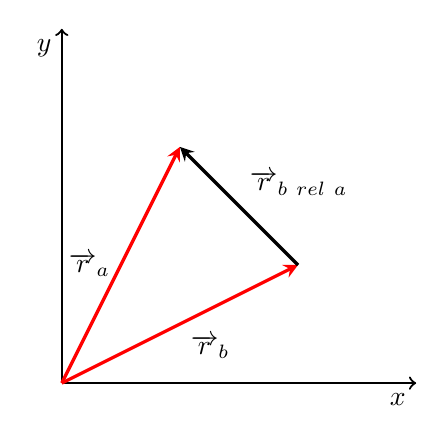
\begin{tikzpicture}[scale=1.5]


\draw[thick,->] (0,0,0) -- (3,0,0) node[anchor=north east]{$x$};
\draw[thick,->] (0,0,0) -- (0,3,0) node[anchor=north east]{$y$};


%draw a vector from origin to point (P) 
\draw[-stealth,very thick,color=red] (0,0) -- (1,2) node[midway,anchor=east,color=black]{$ \overrightarrow{r}_a$};
\draw[-stealth,very thick,color=red] (0,0) -- (2,1) node[midway, anchor=north west ,color=black]{$\overrightarrow{r}_b$};
\draw[-stealth,very thick,color=black] (2,1) -- (1,2) node[midway, anchor=south west ,color=black]{$\overrightarrow{r}_{b\ rel\ a}$};
%\draw[-stealth,very thick,color=black] (1,2) -- (1.2,2.4) node[anchor=south,color=black]{$\hat{r}$};
%\draw[-stealth,very thick,color=black] (1,2) -- (0.6,2.2) node[anchor=east,color=black]{$\hat{\theta}$};


%draw projection on xy plane, and a connecting line
%\draw (0.75,0) arc (0:60:0.75) ;
%\draw (0.25,0.1) node [anchor=south west,color=black]{$\theta$};



\end{tikzpicture}
$$

\vspace{1cm}

\noindent For non-relativistic speeds we assume velocities much slower than the speed of light and can calculate as follows.

$$\overrightarrow{r}_{b\ rel\ a}=\overrightarrow{r}_{a}-\overrightarrow{r}_{b}$$
\vspace{1cm}
$$\overrightarrow{v}_{b\ rel\ a}=\overrightarrow{v}_{a}-\overrightarrow{v}_{b}$$



